\documentclass{yellowpaper}
\usepackage{graphicx}
\usepackage{balance}  % for  \balance command ON LAST PAGE  (only there!)

\begin{document}

\title{Emotiq Yellowpaper}

\numberofauthors{1} 

\author{
\alignauthor
The team\\
       %\affaddr{Emotiq AG}\\
       \email{info@emotiq.ch}
}
\date{22 March 2018}

\maketitle

\begin{abstract}
We are nearing the future where scalability and high transaction throughput will be the baseline for blockchain technology. We are are not there yet and the race for an industrial-strength blockchain foundation is still on. We would like to present Emotiq, a decentralized public blockchain with strong consistency, fast transaction throughput, unlimited horizontal scalability through sharding, strong cryptography, privacy via non-interactive zero-knowledge proofs and natural language smart contracts.
\end{abstract}

\section{Introduction}

Emotiq is a public decentralized blockchain so anyone can join the network, become a validator and earn rewards for maintaining it. Emotiq uses the Proof-of-Stake (PoS) approach and all validators need to post a security bond of a fixed number of tokens which are forfeited if the validator is found cheating.

Emotiq uses a Byzantine consensus protocol with strong consistency which enables all validators to agree on the validity of blocks, without wasting computational power resolving inconsistencies (forks). Clients don?t need to wait more than a few seconds to be certain that a submitted transaction is committed; as soon as it appears in the blockchain, the transaction can be considered confirmed. 

Emotiq provides unlimited horizontal scalability and throughput of thousands of transactions per second through sharding, as well as a cross-shard commit protocol.

Emotiq uses Boneh-Lynn-Shacham (BLS) pairing-based crypto (PBC). This enables short BLS signatures on public keys, as well as hierarchical deterministic wallets with all of the advantages promoted by BIP-32 but without the security risks. 

We also cloak transactions through non-interactive zero-knowledge proofs and purge old and spent transactions. The former provides increased privacy by hiding transaction amounts and the latter drastically reduces the amount of data required to be maintained by validators.

Unlike most technical papers out there, this paper is designed to give the reader a technical overview of the platform using simple and plain language. We start with a look at networking and proceed to token economics and consensus, after which we review confidential transactions, blockchain pruning, real-time transactions validation and other parts of the system. We conclude with a forward outlook.

\section{Networking}
The Emotiq network is composed of full nodes, called validators, and light clients, e.g. those running on mobile devices or in the or browser. Each validator maintains a full copy of the blockchain and associated data structures. Validators participate in the collective signing protocol and respond to queries by light clients. 

Emotiq maintains the core of the network by running a number of validator nodes which both simplifies the bootstrap of new nodes and ensures continuity of the network. The addresses of the core nodes are hard-coded into each release of the Emotiq blockchain software.

Each node keeps a list of addresses of the nodes it knows about (peers) and adds new nodes to the list as it becomes aware of them. A new node starting up connects to one of the core nodes to fetch a list of peers. Each validator node quickly re-broadcasts each received transaction to a random subset of its peers, after only a few light checks. This both ensures that a node cannot be DDOS-ed with transactions to validate and that it does not re-broadcast junk transactions.

To discourage bad actors, we employ a mechanism to both throttle peers and punish peers for bad transactions, etc. by blocking them from further participation in the network.

\section{Consensus}

% Proof-of-Stake, strong consistency

\subsection{Collective Signing}

\subsection{Bias-resistant Distributed Randomness}

\subsection{Leader Election}

\section{Transactions}
UTXO was first introduced by Bitcoin and, unlike Ethereum, aggregates spent and unspent coins, available across multiple wallets, into a single balance. Not only does UTXO offer simplicity, but also drastically increases Emotiq?s scaling capability, by enabling transactions to be processed independently and in parallel.

Emotiq transactions consist, at a minimum, of the sender?s signature and public key, the receiver address or addresses, as well as a smart contract that governs how the transaction may be used.

Emotiq uses zero-knowledge proofs to ensure transaction amounts, among other things, are not visible in the public ledger. For example, although blockchain addresses are represented by random strings, it is currently possible for mapping software to crawl Bitcoin?s ledger for spent and unspent (UTXO) coins, to identify the transactions of a single private key and determine a holder?s total wealth in Bitcoin. While non-interactive zero-knowledge proofs do not prevent such transaction graph analyses, they prevent the tracing party from seeing the amounts being transferred.

Emotiq builds upon MimbleWimble and strong cryptography to ensure that spent transactions can be pruned and new nodes can efficiently validate the blockchain without downloading any old or spent transactions. Unlike with Proof-of-Work (PoW),  where transaction pruning can lower security by lowering the amount of work needed to be redone by an attacker, the approach does present an issue for our PoS blockchain.

% Bulletproofs

\section{Transaction Pruning}


% Cryptographically secure transaction pruning via MimbleWimble


\section{Blocks}
Blocks consist of a header and a list of transactions. The block header contains a hash of the previous block, the collective signature and the list of public keys of co-signers, plus the Merkle root of the transactions stored in the block.

\subsection{Rewards and incentives}

\section{Cryptography}
%%%%%%%%%%%%%%%%%%%%%%%%%%%%%%%%%%%%%%%%%%%%%%%%
\subsection{Pairing-based Cryptography}
Emotiq utilizes advanced bilinear pairing-based cryptography\cite{thesis}\cite{lib} (PBC) for user keying, Boneh-Lynn-Shacham (BLS) Signatures\cite{bls}, fast multi-party signatures, and for Randomness Generation. The advantages of PBC are numerous and include short signatures, fast signature generation, safe deterministic hierarchical wallet keying, and fast multiparty randomness generation.

A bilinear pairing uses pairs of Elliptic Curves, defined over two separate groups, such that their bilinear mappings produce homomorphic encryption in a resulting composite field. If we denote the two curve groups as $G_1$ and $G_2$,  their Tate pairing field $G_T$, and prime order finite field $Z_q$, then their pairing $e(G_1,G_2) \in G_T$ is such that $$e(a \, U, V) = e(U, a \, V)= g^a$$ where $U \in G_1$, $V \in G_2$, $a \in Z_q$, and $g \in G_T$.

In our system, pairings are asymmetric. Group $G_1$ is always the smaller group, with the shortest representation. Pairings are ordered, and must be performed with a $G_1$ element as the first argument, and a $G_2$ element as second. 

Specifically, our $Z_q$ uses 256 bits, $G_1$ was chosen to have a 264-bit representation, $G_2$ has a 520-bit representation, $G_T$ has a 3072-bit representation, and the prime order of the groups is $q \approx  2^{254}$, which gives us roughly $2^{127}$ security.

Private keys belong to the finite field $Z_q$ with the same prime group order. Public keys are generated in $G_2$, and signatures are generated in $G_1$. The embedding degree of our curves is 12, and correspond to {\emph{Type f}} asymmetric pairing curves in Lynn's Thesis\cite{thesis}. Wherever they occur, we use  compressed point representation for group elements from $G_1$ and $G_2$.

The complete specification of the Emotiq cryptosystem requires knowledge of all curve pairing parameters, plus two chosen generators $U \in G_1$, and $V \in G_2$. 

Hash values are first mapped to an element of $Z_q$ before creating points in $G_1$ and $G_2$ as 
$$G_1(H(x)) \equiv Z_q(H(x)) \, U$$ 
and 
$$G_2(H(x)) \equiv Z_q(H(x)) \, V$$

In the following presentation we shall try to adhere to the convention that groups $G_1$ and $G_2$ are additive groups, while $Z_q$ and $G_T$ are both additive and multiplicative. Capitalized symbols denote groups and points from Elliptic curves, while lower cased symbols denote elements of finite fields. Field arithmetic in $Z_q$ is implicitly performed $(mod\,q)$.

%%%%%%%%%%%%%%%%%%%%%%%%%%%%%%%%%%%%%%%%%%%%%%%
\subsection{Boneh-Lynn-Shacham (BLS) Signatures}

BLS signatures are the shortest possible, and enable multisignature generation in just one pass. A BLS signature on message $msg$ is computed as $$Sig = s \, G_1(H(msg))$$ where $H(x)$ is the SHA3/256 hash of its argument, $s \in Z_q$ is the user's secret key value, and $G_1(H(x)) \in G_1$ is the group member that corresponds to that hash value. A signature is always accompanied by the public key of the signer, $P = s \, V$, for generator $V \in G_2$,  producing a signed message as a triple $$(msg, Sig, P)$$

Because of homomorphism we can verify a signature by noting that a valid signature exhibits the pairing relationship 
$$
\begin{align}
    e(Sig,V) &= e(s \, G_1(H(msg)),V)\\
             &= e(G_1(H(msg)), s \, V) \\
             &= e(G_1(H(msg)), P)
\end{align}
$$

And also because of homomorphism, we can easily compute a multi-party signature by simply summing the individual signatures and also summing their corresponding public keys: 
$$e({\sum_i s_i} \, G_1(H(msg)),V) = e(G_1(H(msg)), {\sum_i P_i})$$
producing the collective triple 
$$(msg, {\sum_i sig_i}, {\sum_i P_i})$$

Therefore, during the computation of collective signatures, we need only a single pass through all participants as we gather and sum their signature components. A collective signature appears no different than a single signature.\\

%%%%%%%%%%%%%%%%%%%%%%%%%%%%%%%%%%%%%%%%%%%%%
\subsubsection{Comparison with Schnorr Signatures}
In contrast, conventional Schnorr signatures require two signature values, forming a quadruple with message and public key. For message $msg$ the Schnorr signature is the pair $(R,u)$ of an Elliptic Curve point $R$ and a field value $u$, where $R = r \, G$, for generator point $G$, and 
$$r = H(k_{rand}, msg, P)$$ 
is chosen as a random offset. Finally 
$$u = r + H(R,P,msg)\, s$$ 
The Schnorr signature is validated by checking that 
$$u\, G = R + H(R, P, msg)\, P$$

For collective Schnorr signing, all participants are asked to compute their own commitments $R_i = r_i\, G$. Those values are collected and summed to produce a global challenge value, $c_{glb} = H(\sum_i R_i, \sum_i P_i, msg)$.  Then the participants are asked to produce their $u_i$ values against that global challenge:
$$u_i = r_i + c_{glb} \, s$$
and again the values are summed. Hence collective Schnorr signatures require two interactions with every signer of the message. Network traffic is approximately twice that required for BLS signatures, with a consequent window of opportunity for attackers to spoil the process during the second round.
%%%%%%%%%%%%%%%%%%%%%%%%%%%%%%%%%%%%%%%%%%%%%%%%
\subsection{Cosi Multisignatures}
We use Cosi trees\cite{cosi} to provide scalable, distributed, multisignature generation. Validator nodes are selected from among a group of stakeholder nodes, using random sortition to assign $N$ of them to a position in a Cosi tree. 

A Cosi tree is an n-way tree, where each node in the tree interior is a group leader over $n$ subnodes, each of which may be group leaders over their own subtrees. At any one time, there may be several Cosi trees operating for different purposes, and some nodes might belong to more than one Cosi tree.

When a signature is requested from a Cosi tree, the message is distributed down through the tree to all participant nodes. Each node then attempts to validate the message and decides whether or not to add its BLS signature to the collective signature formed from the sum of all signatures of its subgroup, before passing the augmented signature back up to its parent node in the tree. Accompanying that signature is a composite public key consisting of the sum of participant node public keys, and a bitmap that represents which nodes actually signed the message.

Validation of a message requires varying computation based on the type of message. For randomness generation, it means validating all publicly verifiable quantities and producing decrypted shares. For block validation it means verifying the public keys of all signers of the block, validating all transactions, and so on.

At the top of the tree the bitmap is converted into a list of public keys for all participating nodes, which is used to verify the summed public key, and to gain a census count on how many nodes actually signed the message. That census count is checked against a pBFT threshold of $2 f+ 2$, where $f = \lfloor \frac{N-2}{3} \rfloor$ is the tolerance for Byzantine failures among the nodes, to decide whether the multisignature is acceptable. 
%%%%%%%%%%%%%%%%%%%%%%%%%%%%%%%%%%%%%%%%%%%%%%%%%
\subsection{Consensus using Cosi}
In and of itself, a single pass through a Cosi tree is insufficient to guarantee pBFT. Instead, we perform two passes. The first one sends a message to be validated by all member nodes of the Cosi network. On return the message has acquired some number of signatures. If that number exceeds the requisite pBFT threshold then we will have completed a successful {\em{prepare}} phase of pBFT.

The second pass sends the, now validated, message and its multisignature to all participant nodes in the Cosi network, to ensure that each node has seen the validated multisignature. Their new signatures attest that they will remember this message for future reference in efforts to deny double spending. This corresponds to the {\em{commit}} phase of consensus. Once all Cosi nodes have signed off on the validated message, and if the count remains above the pBFT threshold, the caller of this consensus round can be confident that pBFT consensus has been achieved.
%%%%%%%%%%%%%%%%%%%%%%%%%%%%%%%%%%%%%%%%%%%%%%%%%%
\subsection{Transaction Privacy}
A simple technique for cloaking all transactions in a publicly verifiable manner does not need bilinear pairings, although an algorithm in bilinear pairings can also be developed.\footnote{For single curve computations, we perform in field $Z_q$ and group $G_2$ since that field already has our private keys, and the $G_2$ group has our public keys. Hence the same keying can be used over a single curve algorithm and for all of our pairing cryptography.}

We start with recognizing that a full transaction satisfies the following simple relation:
$$paid = cost + fees + change$$
where $paid$ is the amount tendered in the transaction, $cost$ is the cost of the product or service, $fees$ are transaction fees that must be paid, and $change$ is the amount returned to the buyer, due to overpayment.

Hence, if a spending transaction is rewritten in the form:
$$change - paid = -(cost + fees)$$
then when $(cost + fees)$ is added to this transaction by the seller, the resulting full transaction will show a zero balance. It is very simple to advertise a zero balance, or some function of zero, such that everyone can recognize it.

To provide privacy for the transaction, the numeric value of $(change - paid)$ is homomorphically encrypted to prove that only the sender could have encrypted it, yet the addition of $(cost + fees)$ can be performed and produce the encoding of zero for all to see. 

At the same time, we must also provide cryptographic proofs that the values of $change$ and $paid$ both lie within legitimate range, and that $change < paid$. That is the purpose of Bulletproofs, discussed in the next section.

A buyer cloaks his or her purchase offer by forming a quadruple $(P_{buy}, P_{sell}, t_{buy}, R_{sell})$, for public keys $P_{buy} = s_{buy} \, V \in G_2$, $P_{sell} = s_{sell} \, V \in G_2$, $s_{buy}, t_{buy}, s_{sell} \in Z_q$, and a point on an Elliptic Curve, $R_{sell} \in G_2$, for generator $V \in G_2$ on the curve, given as
$$t_{buy} = \frac{k_{rand} (change - paid)}{s_{buy}} \in Z_q$$
and
$$R_{sell} = k_{rand}\, P_{sell} \in G_2$$
for $k_{rand}$ a random cloaking factor, and buyer's secret key $s_{buy} \in Z_q$.

The random cloaking factor, $k_{rand}$, provides privacy by making each transaction appear different, even when the same currency values are involved. It also protects the secret keys, since the only other relation anyone knows about them comes from the public keys, and there is the ECDLP barrier of difficulty between them.

At the seller's end, we compute
$$C_{sell} = \frac{cost + fees}{s_{sell}} \, R_{sell} \in G_2$$
for seller's secret key $s_{sell} \in Z_q$, and check that
$$t_{buy}\, P_{buy} + C_{sell} = G_2(0)$$
Value $G_2(0)$ is the identity element in the curve group, and easily  recognized by everyone. To accept the transaction, seller publishes the quadruple $(P_{buy}, P_{sell}, t_{buy}, C_{sell})$ so that everyone can verify the same $G_2(0)$ that represents a valid transaction.

The initial purchase offer cloaks its currency values from everyone, including the seller. The final published transaction is also cloaked with the same $k_{rand}$, and so hides all monetary values, except the zero balance that results from the check equation. Nobody but the intended seller can finish the transaction, and the check equation provides undeniable proof that the buyer created the offer. A zero balance proves that enough currency was supplied to cover net cost.

If a zero result is not produced, then it can only mean one or more of three things. First, the seller may be illegitimate and unable to decrypt the $R_{sell}$ value with the secret key, $s_{sell}$. Second the transaction might not have been produced by the indicated buyer, $P_{buy}$. Or finally, the currency amounts may not match the seller's expectations. In any case, such a transaction would never be permitted into the blockchain.
%%%%%%%%%%%%%%%%%%%%%%%%%%%%%%%%%%%%%%%%%%%%%%%
\subsubsection{Privacy without Encryption}
There may be times when the $(cost + fees)$ is publicly known, and there is no seller involved in a transaction. We can still achieve transactional privacy in that case. Simply make the substitutions
\begin{align}
P_{sell} &\to V \in G_2 \notag \\
s_{sell} &\to 1 \notag
\end{align}

The buyer publishes the triple $(P_{buy}, t_{buy}, R)$, where $t_{buy}$ is as before,
$$t_{buy} = \frac{k_{rand} (change - paid)}{s_{buy}} \in Z_q$$
and
$$R = k_{rand}\, V \in G_2$$

Then anyone knowing the value of $(cost + fees)$ can verify the transaction using
$$C = (cost + fees) \, R \in G_2$$
and check that
$$t_{buy}\, P_{buy} + C = G_2(0)$$

The validation relation proves that the buyer formed the purchase offer, and that they forwarded enough money to cover net costs, while still cloaking the values involved. The cloaked values need to be accompanied by range proofs.

%%%%%%%%%%%%%%%%%%%%%%%%%%%%%%%%%%%%%%%%%%%%%%%%%%
%%%%%%%%%%%%%%%%%%%%%%%%%%%%%%%%%%%%%%%%%%%%%%%%%%
\subsection{Bulletproofs}

%%%%%%%%%%%%%%%%%%%%%%%%%%%%%%%%%%%%%%%%%%%%%%%%
\section{Randomness}
Bias-resistant public randomness is a critical component of the Emotiq consensus protocol. Emotiq employs RandHerd, a large-scale distributed protocol that provides publicly-verifiable, unpredictable, and unbiasable randomness against Byzantine adversaries by implementing an efficient, decentralized randomness beacon. RandHerd arranges participants into verifiably unbiased random
secret-sharing groups, which then repeatedly produce random output at predefined intervals. Emotiq uses RandHerd to elect leaders during each block-signing round, as well as to form shard groups.
%%%%%%%%%%%%%%%%%%%%%%%%%%%%%%%%%%%%%%%%%
\subsection{Fast Randomness Generation with PVSS}

The use of BLS Signatures allows an abbreviated form of PVSS randomness generation. Participants in randomness generation are given a list of neighboring group nodes in the network, with whom they carry out a pBFT protocol with publicly verifiable secret sharing (PVSS). 

Within each group, a sharing threshold is set at $t = \lfloor \frac{N}{3} \rfloor + 1$ for group size $N$. Secret random seeds are generated by each participant, then encrypted shares are formed over that secret and distributed to other group members, along with cryptographic proofs on the shares.

For sharing threshold $t$, a random polynomial of order $t-1$ is generated $$p(x) = a_0 + a_1 x + ... + a_{t-1} x^{t-1}$$ with the secret value denoted by $a_0$.  Shares are constructed by computing the value of this polynomial for each member of the group, assigned successive ordinal values, $i = 1 ... N$. The resulting share values, $p(i)$, are then encrypted by multiplying the share value by the public key of each member, $E(share_i) = Z_q(p(i))\, P_i \in G_2$, and proofs are generated by forming a point, $Proof_i = Z_q(p(i)) \,U \in G_1$, for generator $U \in G_1$. 

A vector of shares and a vector of proofs is generated, one element for each member of the group, and these vectors are then transmitted to each group member.
$$(E(share_1), E(share_2), ..., E(share_N))$$
$$ (Proof_1, Proof_2, ..., Proof_N)$$

As with any BLS signature, each share is validated against its proof by checking that the pairings match:
$$ e(Proof_i, P_i) = e(U, E(share_i))$$

Every member of the group can also verify that all shares from another group member were consistently generated from the same sharing polynomial. To do so, we treat the share vector as a codeword from a Reed-Solomon encoding\cite{scrape}, compute a random polynomial of order $N - t - 1$ and use that to compute a test vector from the dual-space of the original share generating polynomial:
$$f(x) = b_0 + b_1 x + ... + b_{N-t-1} x^{N-t-1}$$
$$c_{\perp} = (\lambda_1 f(1), \lambda_2 f(2), ... , \lambda_N f(N))$$
where weights $\lambda_i = \prod_{j \ne i} \frac{1}{i-j}$, for $ i,j = 1...N$.
Then the consistency of the encrypted shares is verified by checking that:
$$\sum_i {c_{\perp}}_i \, Proof_i = G_1(0)$$

This consistency check is absolutely certain for valid sharing vectors, and has an inconsequential probability of failing to detect an improper sharing set given as $\approx 1/q$, or about 1 chance in $2^{254}$. There is a greater likelihood of finding a hash collision in SHA3/256 than in seeing a failure to detect an inconsistent sharing vector.

After performing consistency checks on the sharing set from one group member, the share directed at one node can be decrypted with its secret key to produce a decrypted share, $$G_2(share_i) = \frac{1}{s_i}E(share_i) \in G_2$$ for secret key $s_i \in Z_q$.

This decrypted share is then broadcast to all group members. Decrypted shares can be verified from the pairing relation:
$$ e(Proof_i, V) = e(U, G_2(share_i))$$

As soon as a sharing threshold number, $(n \ge t)$, of decrypted shares has been seen for any one sharing set, the secret randomness from that set can be discovered via Lagrange interpolation:
$$G_2(random) = \sum_i G_2(share_i) \prod_{j \ne i} \frac{i}{i-j}$$

Finally, after a supermajority of sharing sets has been decrypted, $(n \ge 2 \lfloor \frac{N}{3} \rfloor + 1)$, their randomness is combined as a simple sum in $G_2$, and forwarded to all other groups.
$$G_2(random_{grp}) = \sum_i G_2(random_i)$$

Proof of group randomness comes from the sum of Lagrange interpolations of the individual proof sets.
Final randomness results from a supermajority sum of randomness obtained from each group, and its proof results from the sum of group proofs. 

So the use of pairing-based cryptography shows great benefits, not only in minimizing network traffic, and by making immediate commitments to portions along the way, and also from the fact that proofs are so easily generated as simple sums of existing proofs.

Timing tests show that this approach scales linearly with number of group participants, ranging from about 5 seconds for 32 group members, to about 7 minutes for 1024 group members, on an ordinary iMac with an Intel i7 processor. The timings are dominated by compute load, not network communications.

\begin{figure}[h!]
  \centering
  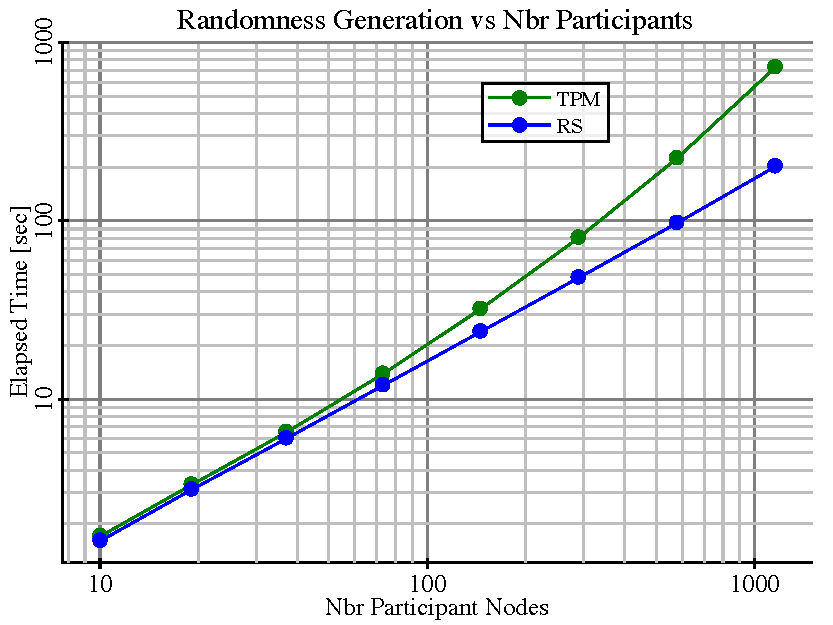
\includegraphics[width=3in]{randtimings}
  \caption{ Comparison of performance between the TPM Method and the Reed-Solomon interpretation of proof vectors.}
  \label{fig:randtimings}
\end{figure}

%%%%%%%%%%%%%%%%%%%%%%%%%%%%%%%%%%%%%%%%%%%%%

\subsubsection{The TPM Method}
There is an alternate method for generating randomness with PVSS, which I call the TPM Method.\cite{tpm}\footnote{The paper has an error wherein it specifies that encrypted shares should be formed as the product of the share value and the generator of the curve. That is incorrect, as the encryption needs to incorporate information about the target node keying. It seems likely that the error crept in by way of fractured translation to English. I found the nomenclature terribly inconsistent and confusing.} It performs the same share generation procedure as seen above, but instead of sending along a vector of proofs on each encrypted share, it sends along proofs on the sharing polynomial coefficients, $a_i, i = 0..t-1$ using $Aproof_i = a_i U$ for generator $U \in G_1$.

Then, at each receiving node, the shares are verified by computing the sums
$$ Proof_i = \sum_{j=0..t-1} i^j\, Aproof_j, i = 1..N$$
Then the pairing relation is checked
$$e(Proof_i, P_i) = e(U,E(share_i))$$

These proof sums correspond directly to the proofs presented in the previous section. And they also directly verify that every encrypted share came from the same polynomial. One advantage of this method is that instead of transmitting $2 N$ vector elements, we now only need to transmit $N+t$ elements.

However, we now also need to supply these proof sums along with any decrypted shares that we compute, and the method scales super-linearly. Timing tests have shown it to be a hair slower than the first method for $N=32$, and about half as fast when $N=1024$. But the method is equivalent in its information content, and every bit as secure.
%%%%%%%%%%%%%%%%%%%%%%%%%%%%%%%%%%%%%%%%%%%%%%%
\subsection{Verifiable Random Functions}
A verifiable random function (VRF)\cite{vrf2} uses a pseudo-random function (PRF) in such a way as to furnish proof that the resulting pseudo-random value came from a specific seed value mixed with the creator's secret key. And even though a secret key was involved in the generation of randomness, anyone can duplicate the calculation by knowing only the seed value and creator's public key. We follow the work of Dodis and Yampolskiy\cite{vrf}, to provide a PRF as follows:

For arbitrary input seeding values, form the hash $H(seed)$ using SHA3/256. This converts arbitrary objects of any length into a 256-bit random-like, but reproducible, pattern. Then map that hash value into our $Z_q$ field, which has dimension $q = |Z_q| \approx 2^{254}$, to produce $x = Z_q(H(seed))$.

Output of the VRF is a pseudo-random value in the pairing field (3072 bits) 
$$y = VRF(x, s) = e(U,V)^{1/(x + s)} \in G_T$$ 
for secret key $s \in Z_q$,  generators $U \in G_1$, $V \in G_2$, and with proof 
$$R = \frac{1}{x+s}\,U \in G_1$$ 

Output of the VRF is the quadruple $(seed, x, y, R)$, i.e., the original seed, the seed deterministically reduced to an element of $Z_q$, the output of the VRF computation, and the point in $G_1$ that represents the proof.

Verification of proof checks the pairing $$e(R, x \, V + P) = e(U,V)  \in G_T$$ for public key $P = s \, V \in G_2$, and to verify that $$y = e(R,V)$$ and that $$x = Z_q(H(seed))$$
%%%%%%%%%%%%%%%%%%%%%%%%%%%%%%%%%%%%%%%%%%%%%%%%%%%
\subsection{Safe Hierarchical Keying}

In current blockchain designs which utilize simple Elliptic Curve cryptography, the possibility of producing subkeys from a master public key is presented. But that is wholly unsafe in the event that a decryption key is also generated for a derived public key. A simple bit of finite field arithmetic is all it takes to discover the original master private key.

With PBC we can safely generate both public and private keys without exposing our master private key. This is also known as Identity-Based Encryption (IBE). But unlike conventional presentations of IBE, we do not rely on a trusted third party for the generation of our keying. Rather, we view the master key holder as the only entity that should be entitled to generate new decryption keys. 

Anyone can generate new public keys at any time, based on previously known public keys.
But in order to obtain a decryption key for the new public keys, you must ask the primary secret key holder for a decryption key. Doing so puts the primary key holder at no risk for exposing his or her private key.

A new public key can be generated by asking for a subkey of a given public key, using an arbitrary identity value to identify that subkey. The new public key is computed as 
$$ P_{id} = Z_q(H(id)) \, V + P$$ 
for identity $id$, generator $V \in G_2$, public key $P \in G_2$, and where $Z_q(H(id)) \in Z_q$ is the element of the field that corresponds to the hash of the supplied identity. 

You can use this public key to encrypt a message by making use of the hash of a pairing value as an XOR mask against a message $$E(msg) = msg \oplus H(g^r)$$ where $r = Z_q(H(msg, id)) \in Z_q$, and pairing element 
$$g^r = e(U, r \, V)$$
for generator $U \in G_1$, generator $V \in G_2$. The message is transmitted as the triple $(E(msg), R, id)$, with $R = r \, P_{id} \in G_2$.

In order to produce a decryption key for that new public key, the primary key holder computes $$S_{id} = \frac{1}{s + Z_q(H(id))} \, U \in G_1$$ for secret key $s \in Z_q$. Producing a decryption key in $G_1$ ensures, by difficulty of ECDLP, that our master private key remains safe against exposure.

Homomorphism allows us to see that the pairings 
$$
\begin{align}
    e(S_{id}, R) &= e(\frac{1}{s + Z_q(H(id))}\, U, r\,(Z_q(H(id)) \, V + P)) \\
    &= e(U, r\, V) = g^r
\end{align}$$ 
which allows us to recreate the XOR mask and decrypt to the original message 
$$msg = E(msg) \oplus H(g^r)$$ 

Verification of the message is done by computing $r = Z_q(H(msg, id))$ and checking that 
$$r\, (Z_q(H(id))\, V + P) = R \in G_2$$

In this form, a new private key cannot be used to sign messages in the usual manner as for BLS signatures with the master private key, because we have $P_{id} \neq s_{id} \, V$. But it does furnish a way to encrypt and decrypt messages by using the hash of the pairing result. This technique has been dubbed SAKKE by its authors Sakai-Kasahara\cite{sakke}. We have extended SAKKE encryption to indefinite length by using successive SHA3 hashes on the pairing field result and an increasing index value.
%%%%%%%%%%%%%%%%%%%%%%%%%%%%%%%%%%%%%%%%%%%%%%

% ensure same length columns on last page (might need two sub-sequent latex runs)
\balance

% The following two commands are all you need in the
% initial runs of your .tex file to
% produce the bibliography for the citations in your paper.
\bibliographystyle{abbrv}
% \bibliography{yellowpaper}  

\begin{thebibliography}{99}

\bibitem{scrape}Ignacio Casudo and Bernardo David, 
{\em{ SCRAPE: Scalable Randomness Attested by Public Entities}} 

\bibitem{vrf}Yevgeniy Dodis and Aleksandr Yampolskiy, 
{\em{A Verifiable Random Function With Short Proofs and Keys}}

\bibitem{thesis} Ben Lynn, PhD Thesis, 
{\em{On the Implementation of Pairing-Based Cryptosystems}}, June 2007

\bibitem{lib} Ben Lynn, PBC Library, 
https://crypto.stanford.edu/pbc/download.html

\bibitem{bls} Ben Lynn, 
{\em{BLS Signatures}}, 
https://crypto.stanford.edu/pbc/manual/ch02s01.html

\bibitem{vrf2}Silvio Micali, Michael Rabin, Salil Vadhan, 
{\em{Verifiable Random Functions}}

\bibitem{sakke}Sakai-Kasahara, 
{\em{IETF RFC 6508 Sakai-Kasahara Key Encryption (SAKKE)}} 

\bibitem{cosi}Ewa Syta, Iulia Tamas, Dylan Visher, David Isaac Wolinsky, Philipp Jovanovic, Linus Gasser, Nicolas Gailly, Ismail Khoffi, Bryan Ford, 
{\em{Keeping Authorities ``Honest or Bust'' with Decentralized Witness Cosigning}}

\bibitem{randhound} Ewa Syta, Philipp Jovanovic, Eleftherios Kokoris Kogias, Nocals Gailly, Linus Gasser, Ismail Khoffi, Michael J. Fisher, Bryan Ford, 
{\em{Scalable Bias-Resistant Distributed Randomness}}

\bibitem{tpm} Youlian Tian, Changgen Peng, Jianfeng Ma, 
{\em{Publicly Verifiable Secret Sharing Scheme Using Bilinear Pairings}}

\end{thebibliography} 
\end{document}
